\documentclass[convert={density=300, outext=.png}, border=0pt]{standalone}

\usepackage[utf8]{inputenc}
\usepackage{tikz}
\usepackage{verbatim}
\usepackage{ulem}

\usetikzlibrary{arrows, positioning}

\begin{document}

	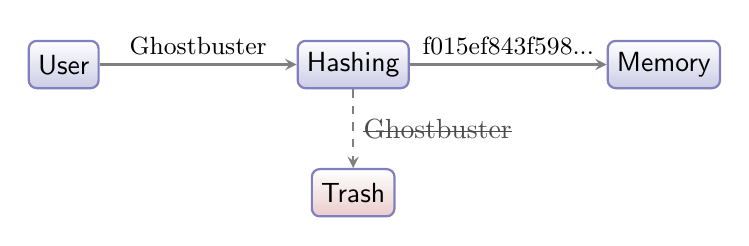
\begin{tikzpicture} [node distance=2.5cm,
		% define styles
		basicnodestyle/.style={
			% The shape:
			rectangle,
			% The size:
			minimum size=6mm,
			% The border:
			thick,
			draw=blue!50!black!50, % 50% blue and 50% black
			% The filling:
			top color=white, % a shadi,ng that is white at the top...
			bottom color=blue!50!black!20, % and something else at the bottom
			% Corners
			rounded corners=1.0mm,
			% Font
			font=\sffamily
		},
		trashnodestyle/.style={
			% The shape:
			rectangle,
			% The size:
			minimum size=6mm,
			% The border:
			thick,
			draw=blue!50!black!50, % 50% blue and 50% black
			% The filling:
			top color=white, % a shadi,ng that is white at the top...
			bottom color=red!60!black!20, % and something else at the bottom
			% Corners
			rounded corners=1.0mm,
			% Font
			font=\sffamily
		},
		arrow/.style={
			->,
			% Thickness
			thick,
			>=stealth,
			% Color
			black!50,
			text=black,
			font=\small
		},
		arrowtrash/.style={
			->,
			dashed,
			% Thickness
			thick,
			>=stealth,
			% Color
			black!50,
			text=black!70,
		}]
		% end of style definition
		
		% draw nodes
		\node (iUser) [basicnodestyle] {User};
		\node (iHashing) [basicnodestyle, right = of iUser] {Hashing};
		\node (iMemory) [basicnodestyle, right = of iHashing] {Memory};
		\node (iTrash) [trashnodestyle, below = of iHashing, yshift = 1.5cm] {Trash};		
		
		% connect nodes
		\draw [arrow] (iUser) -- node[anchor=south] {Ghostbuster} (iHashing);
		\draw [arrow] (iHashing) -- node[anchor=south] {f015ef843f598...} (iMemory);
		\draw [arrowtrash] (iHashing) -- node[anchor=west] {\sout{Ghostbuster}} (iTrash);
	\end{tikzpicture}
	
\end{document}

% use pdflatex -shell-escape password_certification_creation.tex to compile this into png
